\documentclass[tikz,border=10pt]{standalone}

\begin{document}
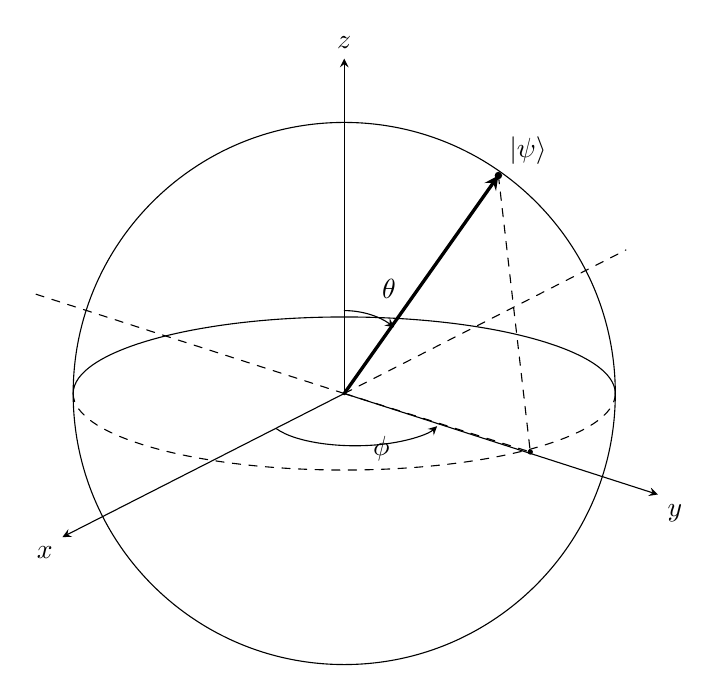
\begin{tikzpicture}[scale=1.35, line cap=round, line join=round, >=stealth]

  \coordinate (O) at (0,0);
  \coordinate (X) at (-2.65,-1.35);
  \coordinate (Y) at (2.95,-0.95);
  \coordinate (Z) at (0,3.15);
  \coordinate (Xp) at (2.65,1.35);
  \coordinate (Yp) at (-2.95,0.95);
  \coordinate (P) at (1.45,2.05);
  \coordinate (Q) at (1.75,-0.55);

  \fill[white] (O) circle (2.55);

  \draw[thin] (O) circle (2.55);
  \draw[thin, dashed] (-2.55,0) arc[start angle=180,end angle=360,x radius=2.55,y radius=0.72];
  \draw[thin] (2.55,0) arc[start angle=0,end angle=180,x radius=2.55,y radius=0.72];

  \draw[->, thin] (O) -- (X) node[below left] {$x$};
  \draw[->, thin] (O) -- (Y) node[below right] {$y$};
  \draw[->, thin] (O) -- (Z) node[above] {$z$};

  \draw[thin, dashed] (O) -- (Xp);
  \draw[thin, dashed] (O) -- (Yp);

  \draw[->, very thick] (O) -- (P) node[above right] {$|\psi\rangle$};

  \draw[thin, dashed] (P) -- (Q);
  \draw[thin, dashed] (O) -- (Q);

  \draw[thin, ->] (0,0.78) arc[start angle=90,end angle=53,x radius=0.78,y radius=0.78];
  \node at (0.42,0.98) {$\theta$};

  \draw[thin, ->] (-0.64,-0.33) arc[start angle=205,end angle=340,x radius=0.82,y radius=0.28];
  \node at (0.35,-0.52) {$\phi$};

  \fill (O) circle (0.018);
  \fill (P) circle (0.035);
  \fill (Q) circle (0.025);

\end{tikzpicture}
\end{document}
